% debut d'un fichier latex standard
\documentclass[a4paper,12pt,twoside]{article}

% Pour les unités SI
\usepackage{siunitx}
% pour l'inclusion de figures en eps,pdf,jpg
\usepackage{graphicx}
% quelques symboles mathematiques en plus
\usepackage{amsmath}
% le tout en langue francaise
%\usepackage[english]{babel}
% on peut ecrire directement les caracteres avec l'accent
% a utiliser sur Linux/Windows
\usepackage[utf8]{inputenc}
\usepackage[T1]{fontenc}

% pour faire des systèmes d'équations
\usepackage{systeme}

% a utiliser sur le Mac
%\usepackage[applemac]{inputenc}
% pour l'inclusion de links dans le document 
\usepackage[colorlinks,bookmarks=false,linkcolor=blue,urlcolor=blue]{hyperref}
\usepackage{subcaption}
\paperheight=297mm
\paperwidth=210mm

\setlength{\textheight}{235mm}
\setlength{\topmargin}{-1.2cm} % pour centrer la page verticalement
%\setlength{\footskip}{5mm}
\setlength{\textwidth}{15cm}
\setlength{\oddsidemargin}{0.56cm}
\setlength{\evensidemargin}{0.56cm}

\pagestyle{plain}

% quelques abreviations utiles
\def \be {\begin{equation}}
\def \ee {\end{equation}}
\def \dd  {{\rm d}}

\newcommand{\mail}[1]{{\href{mailto:#1}{#1}}}
\newcommand{\ftplink}[1]{{\href{ftp://#1}{#1}}}
%
% latex SqueletteRapport.tex      % compile la source LaTeX
% xdvi SqueletteRapport.dvi &     % visualise le resultat
% dvips -t a4 -o SqueletteRapport.ps SqueletteRapport % produit un PostScript
% ps2pdf SqueletteRapport.ps      % convertit en pdf

% pdflatex SqueletteRapport.pdf    % compile et produit un pdf

% ======= Le document commence ici ======

\begin{document}
% Le titre, l'auteur et la date
\title{Particle in an electromagnetic field\\{\small Physique Numérique I}\\{\small 2nd report}}
\date{\today}
\author{Delphine Martres and Damien Korber\\{\small \mail{delphine.martres@epfl.ch} and \mail{damien.korber@epfl.ch}}}
\maketitle
\tableofcontents % Table des matieres

% Quelques options pour les espacements entre lignes, l'identation 
% des nouveaux paragraphes, et l'espacement entre paragraphes
\baselineskip=16pt
\parindent=15pt
\parskip=5pt



%%%% ON COMMENCE A ECRIRE D'ICI

\section{Introduction}


\section{Analytic computations}
\subsection{Establishment of the linear equation system}
After some computations that can be found in annex \ref{ann:dev-eq-diff}, the system \ref{eq:equa-diff} results.

\begin{equation}
\systeme*{m\ddot{x} = Bq\dot{y}, m\ddot{y} = qE - Bq\dot{x}}
\label{eq:equa-diff}
\end{equation}

The equation on $z$ axis is neglected because no informations can be obtained from it.

\subsection{Analytics solutions with an null electric field}

\subsection{Center of cercle for a particular radius}

\section{Study of three numerical methods}
% Faire le 2.2 ii) en plusieurs sous parties
\section{Applications}
\subsection{Dérive $E\times B$} %TODO: Traduire "Dérive"
In this experiement, the proton is now subjected to an electric field $E=\SI{6d4}{\volt\per\meter}$, as well as a constant magnetic field $B_0 = \SI{3}{\tesla}$.
The proton starts with an initial velocity of $v_{0x}=\SI{0}{\meter\per\second}$ and $v_{0y}=\SI{4d5}{\meter\per\second}$, and the simulation will last the time it take for the proton to end five revolutions.
\subsubsection{Convergence study}
This section focuses on a convergence study of all three methods used in this experiment, and will compare them.
\begin{figure}[h]
\centering
\begin{subfigure}[c]{0.45\textwidth}
	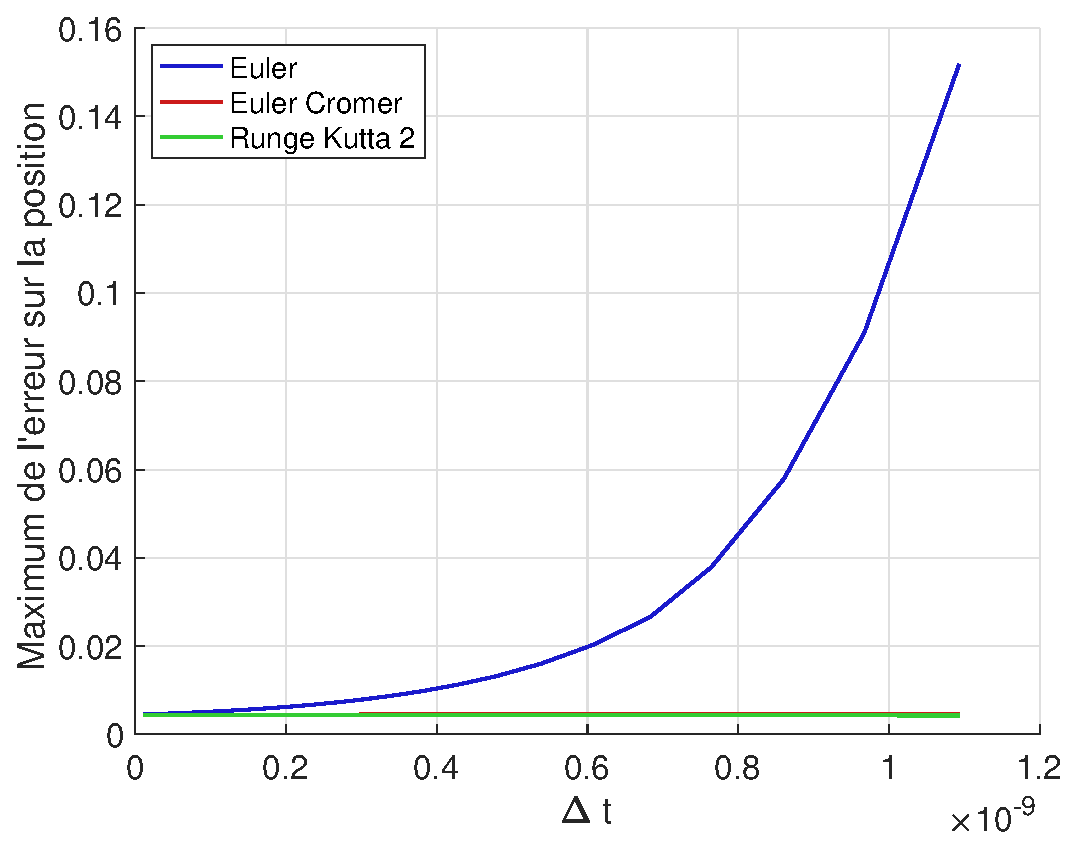
\includegraphics[width=\textwidth]{graphs/app1_conv_ALL.eps}
	\caption{Convergence graph where three methods are drawn.}
	\label{fig:app1-conv-ALL}
\end{subfigure}
~
\begin{subfigure}[c]{0.45\textwidth}
	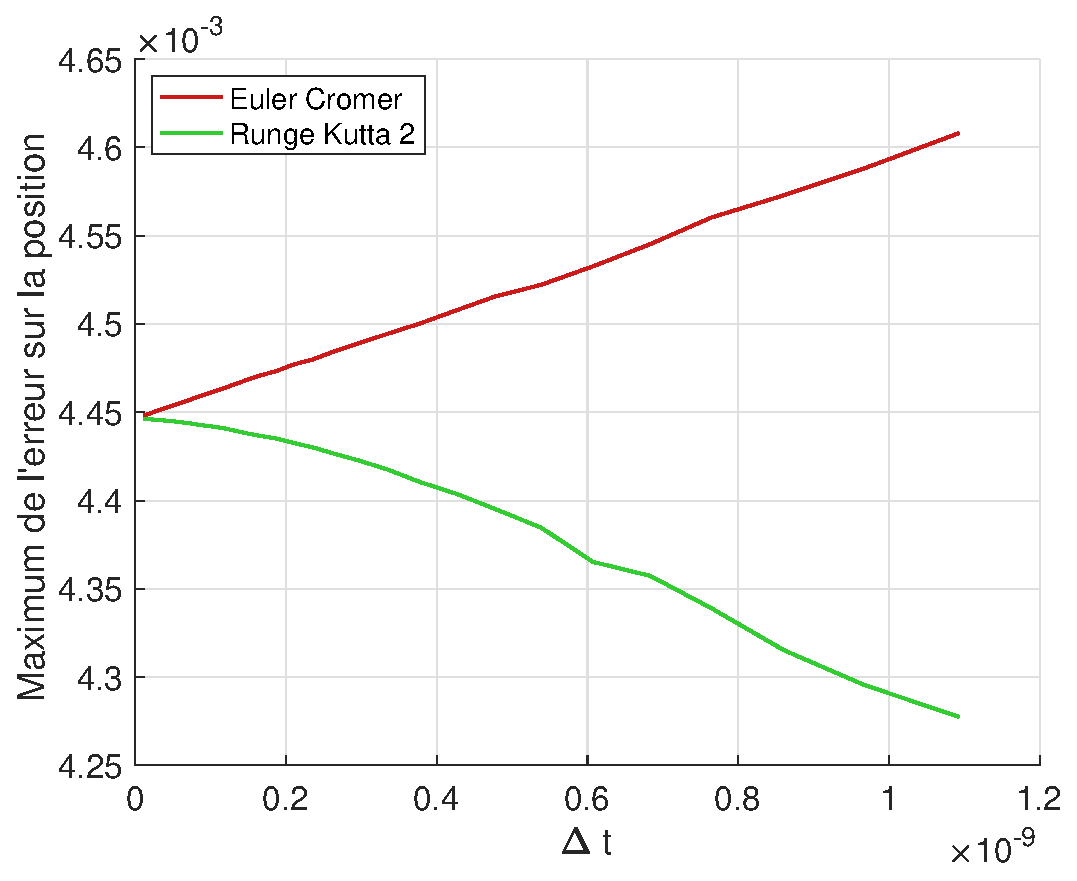
\includegraphics[width=\textwidth]{graphs/app1_conv_noEuler.eps}
	\vfill
	\caption{Convergence graph where Euler's method isn't drawn for readability reasons.}
	\label{fig:app1-conv-noEuler}
\end{subfigure}
\end{figure}

In the figure \ref{fig:app1-conv-ALL}, the main information is fact that Euler's method is not appropriate for this simulation.
The error explodes really quickly, and just keep increasing.
The problem with this figure, is that the others methods can not be analysed.
The figure \ref{fig:app1-conv-noEuler} fixes the problem by focusing on the others methods.
%TODO: Vérifier que l'analyse est encore à jour.
This second figures shows the stability of both methods.
Euler-Cromer clearly is better than Euler's one.
But the error seems to keep increasing, which is bad for long simulation.
Aside from that, the method can be used for small simulation of the same kind.
On the other hand, Runge-Kutta of order 2 is a good option.
The main difference between this method and the two others is the stability.
In this case, the error decreases, which implies stability.
For long simulation, Runge-Kutta of second order is a good option for this kind of simulation.




\subsubsection{Analysis of simulations}
% Faire le 2.3 ii)

\subsubsection{Proton in an accelerated referential}

\subsubsection{Dérive $\nabla B$} %TODO: Traduire "Dérive"

\section{Further analysis...}

\appendix
\section*{Annexes}
\addcontentsline{toc}{section}{Annexes}

\section{Differential equation development} \label{ann:dev-eq-diff}
The mass of the proton is so small, that the gravitational force is ignored in these experiments.
Then the only force remaining is Lorentz's force.

\begin{equation}
	\vec{F}_L = q(\vec{E} + \vec{v}\times\vec{B})
	\label{eq:lorentz-force}
\end{equation}

Using Newton's second law, three equations results.

\begin{align*}
	\Sigma\vec{F}^{ext} &= m\vec{a} \\
	\vec{F}_L &= m\vec{a}\\	
	q(\vec{E} + \vec{v}\times\vec{B}) &= m\vec{a} \\
	q\left( \begin{pmatrix} 0\\ E\\ 0\\ \end{pmatrix} + \begin{pmatrix} \dot{x}\\ \dot{y}\\ 0\\ \end{pmatrix} \times \begin{pmatrix} 0\\ 0\\ B\\ \end{pmatrix}\right) &= m\begin{pmatrix} \ddot{x}\\ \ddot{y}\\ \ddot{z}\\ \end{pmatrix} \\
	\frac{q}{m}\begin{pmatrix} B\dot{y}\\ E - B\dot{x}\\ 0 \end{pmatrix} &= \begin{pmatrix} \ddot{x}\\ \ddot{y}\\ \ddot{z}\\ \end{pmatrix}
\end{align*}

The last equation is not useful for what is about to come. 
The system of differential equation resulting is equation \ref{eq:equa-diff}.

\end{document}